\documentclass{article}

% Recommended, but optional, packages for figures and better typesetting:
\usepackage{microtype}
\usepackage{graphicx}
\usepackage{subfigure}
\usepackage{booktabs} % for professional tables
\usepackage{amsmath}
\usepackage{amsfonts}
\usepackage{multirow}

% hyperref makes hyperlinks in the resulting PDF.
% If your build breaks (sometimes temporarily if a hyperlink spans a page)
% please comment out the following usepackage line and replace
% \usepackage{icml2018} with \usepackage[nohyperref]{icml2018} above.
\usepackage{hyperref}

% Attempt to make hyperref and algorithmic work together better:
\newcommand{\theHalgorithm}{\arabic{algorithm}}

% Use the following line for the initial blind version submitted for review:
%\usepackage{icml2018}

% If accepted, instead use the following line for the camera-ready submission:
\usepackage[accepted]{icml2018}

% The \icmltitle you define below is probably too long as a header.
% Therefore, a short form for the running title is supplied here:
%\icmltitlerunning{}

\begin{document}

\twocolumn[
\icmltitle{Genetic Algorithm for Weighted 3-SAT Problem}

% It is OKAY to include author information, even for blind
% submissions: the style file will automatically remove it for you
% unless you've provided the [accepted] option to the icml2018
% package.

% List of affiliations: The first argument should be a (short)
% identifier you will use later to specify author affiliations
% Academic affiliations should list Department, University, City, Region, Country
% Industry affiliations should list Company, City, Region, Country

% You can specify symbols, otherwise they are numbered in order.
% Ideally, you should not use this facility. Affiliations will be numbered
% in order of appearance and this is the preferred way.
\icmlsetsymbol{equal}{*}

\begin{icmlauthorlist}
\icmlauthor{Ond\v{r}ej Podsztavek}{fit}
\end{icmlauthorlist}

\icmlaffiliation{fit}{
Faculty of Information Technology, Czech Technical University in Prague,
Prague, Czech Republic
}

\icmlcorrespondingauthor{Ond\v{r}ej Podsztavek}{podszond@fit.cvut.cz}

% You may provide any keywords that you
% find helpful for describing your paper; these are used to populate
% the "keywords" metadata in the PDF but will not be shown in the document
\icmlkeywords{genetic algorithm, SAT problem}

\vskip 0.3in
]

% this must go after the closing bracket ] following \twocolumn[ ...

% This command actually creates the footnote in the first column
% listing the affiliations and the copyright notice.
% The command takes one argument, which is text to display at the start of the footnote.
% The \icmlEqualContribution command is standard text for equal contribution.
% Remove it (just {}) if you do not need this facility.

\printAffiliationsAndNotice{}  % leave blank if no need to mention equal contribution
%\printAffiliationsAndNotice{\icmlEqualContribution} % otherwise use the standard text.

\begin{abstract}
TODO abstract.
\end{abstract}

\section{Goal}

This work aims to use a genetic algorithm to solve as wide spectrum of
weighted 3-SAT problems defined in next section~\ref{problem} as possible.
Therefore, the task consists of finding appropriate setting of genetic
algorithm's parameters.

\section{Weighted 3-SAT Problem}
\label{problem}

This section defines weighted 3-SAT problem which is of same difficulty
as Boolean satisfiability (SAT) problem.
SAT problem is proven to be NP-complete problem
which means that all problems in the complexity class NP are at most
as difficult to solve as SAT.~\cite{cook1971}

Given a Boolean formula $F: \mathbb{B}^n \to \mathbb{B}$,
$\mathbb{B} = \{0, 1\}$ in conjunctive normal form with $n$ variables
$X = (x_1, x_2, \dots, x_n) \in \mathbb{B}^n$
where each clause has exactly 3 literals.
Moreover, there are integer weights
$W = (w_1, w_2, \dots, w_n) \in \mathbb{N}$.
Find values $Y = (y_1, y_2, \dots, y_n) \in \mathbb{B}^n$ of variables from $X$
such that $F(Y) = 1$
and sum of weight of variable that has value 1 is maximal.

\subsection{Instances}

For experimental purpose of this work uniform random 3-SAT instances
from SATLIB Benchmark Problems~\cite{hoos2000} are going to be used.
Since genetic algorithms is \textit{incomplete algorithm}\footnote{Incomplete
algorithms for SAT are able to decide if a given formula is satisfiable by
finding a truth assignment
but they cannot detect contradictory formulas
thus ascertain unsatisfiability.~\cite{ellerweg2004}}
only satisfiable instances are included.

The instances are in DIMACS format
which means that they do not contain weights so they are uniformly randomly
generated from set of natural numbers less or equal than 1024.
The upper bound should affect the fitness of an individual
therefore such arbitrary number was chosen.

In order to measure performance of a genetic algorithm
there is a need differently difficult formulas.
A number of paper have claimed that most randomly generated instances are
not that difficult.
But it was empirically found that 3-SAT difficulty depends on ratio of
number of clauses and variables $\frac{m}{n}$.
The most difficult instances has about 4.3 times more clauses than variables.
\cite{selman1996}

Instances from SATLIB Benchmark Problems have usually the highest difficulty.
For example, there are instances with 218 clauses and 50 variables
giving clauses-to-variables ratio of 4.36.
Creation of easier instances can be done by leaving out clauses
which is going to lower the ratio and not affect satisfiability.

\subsection{Testbed}
\label{testbed}

This subsection describes the instances used for experimental evaluation.
As mentioned in previous subsection only satisfiable instances are included
and difficulty is reduced by leaving out certain number of clauses.
It was chosen to test on instances with 50 variables of four difficulties ratios
1.00, 2.12, 3.24 and 4.36.
For each difficulty there is 100 instances.
Table~\ref{testbed-table} summarizes the testbed.

\begin{table}[ht]
\caption{Properties of testbed used for experiments.}
\label{testbed-table}
\vskip 0.15in
\begin{center}
\begin{small}
\begin{sc}
\begin{tabular}{rrrr}
\toprule
Ratio & Variables & Clauses & Instances \\
\midrule
1.00 & 50 & 50  & 30 \\
2.12 & 50 & 106 & 30 \\
3.24 & 50 & 162 & 30 \\
4.36 & 50 & 218 & 30 \\
\bottomrule
\end{tabular}
\end{sc}
\end{small}
\end{center}
\vskip -0.1in
\end{table}

\section{Genetic Algorithm}

The idea of genetic algorithms is to evolve a population of solutions
to a given problem using operators inspired by natural genetic variation
and natural selection.
\cite{mitchell1996}

There is no rigorous definition of genetic algorithm but most methods
have at least in common populations of chromosomes,
selection according to fitness, crossover to produce new offspring
and random mutation of new offspring.
\cite{mitchell1996}

The term \textit{chromosome} refers to a solution to a problem
which is encoded as a bit string
and can be thought of as points in the search space of solutions.
The \textit{genes} are either single or short blocks bits
that encode a particular element of the solution.
An \textit{allele} is 0 or 1 in bit string.
Mostly genetic algorithms employ \textit{single-chromosome haploid} individuals.
The \textit{genotype} of an individual is the configuration of bits
in its chromosome.
\cite{mitchell1996}

The simplest form of genetic algorithm involves three types of operators.
\textit{Selection} in operator which selects chromosomes in the population for
reproduction.
The fitter the chromosome the more it is likely to be selected.
\textit{Crossover} randomly chooses a position in a chromosome
and exchange the subsequences before and after the position between
two chromosomes to create two new offspring.
\textit{Mutation} randomly flips some bits in a chromosome.
\cite{mitchell1996}

The algorithm processes population of chromosomes successively replacing
one population with another (see algorithm~\ref{alg:ga}).
Genetic algorithm requires a fitness function that assigns a score to
each chromosome in the current population.
The chromosome's fitness depends on how well the chromosome solves given
problem.
\cite{mitchell1996}

\begin{algorithm}[hb]
\caption{Genetic Algorithm~\cite{eiben2003}}
\label{alg:ga}
\begin{algorithmic}
\STATE initialize population with random individuals
\STATE evaluate each individual
\WHILE{terminal condition is not satisfied}
\STATE select parents
\STATE recombine pairs of parents
\STATE mutate the resulting offspring
\STATE evaluate new individuals
\STATE select individuals for next generation
\ENDWHILE
\end{algorithmic}
\end{algorithm}

\section{Implementation}

The implementation is in Python 3.6 programming language
and is based on DEAP framework~\cite{fortin2012}.

Chromosomes representation for weighted 3-SAT problem is straight forward.
A chromosome is represented as Python's list of $n$ numbers 0 or 1.
If there is 1 resp. 0 at position $i$ it means that $x_i$ is set to 1 resp. 0.

The skeleton of implemented genetic algorithm is the same as
in algorithm~\ref{alg:ga}.
Population size is fixed through all generation.

In order to stop the evolution of population advantage of
\textit{early stopping} is taken.
This mechanism works based on average fitness of population increase.
If population's average fitness does not increase by a certain amount
during given number of generation the evolution is terminated.

Last commonly used method applied is \textit{elitism}.
This method puts chosen number of elite individuals with best fitness
from previous generation to next generation.

\section{Experiments}

This section presents results of experiments on testbed
shown in section~\ref{testbed}.
Goal is to find suitable parameters
which can perform best on this testbed
and so on wide spectrum of weighted 3-SAT instances.
Experiments were carried out on Intel Core i5-3337U CPU (1.80GHz).

Default parameters are chosen according to proposition in~\cite{dejong1975}.
Population size is 100 individuals, roulette selection,
one point crossover with rate 0.6 per a pair of parents
and mutation rate of value 0.001 per a bit.
Moreover, one elite individual is moved to next generation
and evolution is stopped
if average fitness of last 100 generation does not increase by more than 1.

\subsection{Fitness Function}

Fitness function employed in this work is derived from MAX-SAT fitness
function~\cite{dejong1989} after reading \cite{gottlieb2002}
and \cite{ellerweg2004}.
MAX-SAT problem is concern with maximizing number of satisfied clauses.
Thus it fitness function is the number of satisfied clauses:

$$f_{\text{MAX-SAT}}(Y) = c_1(Y) + \dots + c_m(Y),$$

where $m$ is the number of clauses and $c_i(x)$ is the truth value of the $i$th
clause.

For purpose of weighted 3-SAT problem the MAX-SAT fitness function is
incorporated into fitness function $f$
which value is the sum of weights of variables of value 1
if the formula is satisfied ($F(Y) = 1$)
else it is value of MAX-SAT fitness function $f_{\text{MAX-SAT}}(Y)$
subtracted by total number of clauses $m$:

$$
f(Y) = 
\begin{cases} 
    \sum_{i = 1}^m y_i w_i & \text{if } F(Y) = 1, \\
    f_{\text{MAX-SAT}}(Y) - m & \text{if } F(Y) = 0,
\end{cases}
$$

where $y_i$ is value of $i$th variable, $w_i$ is the weight of $i$th
variable and $m$ is the number of clauses in formula $F$.

\subsection{Basic Evaluation}

This subsection present results of default parameters setting described above.
It shows very poor performance
because it is able to satisfy only easy instances
and also is not that robust.

Table~\ref{result-table} contains success rate which is defined ratio
of satisfied formulas to number of formulas
in corresponding difficulty category.
Then, there is an average number of unsatisfied clauses.

It is obvious that basically parameterized genetic algorithm has problem
with finding chromosome which satisfy non-trivial formulas.
It shows for how many formulas the algorithm was able to find satisfiable
assignment and if it was not able what is the average number of unsatisfied
clauses.

\begin{table}[ht]
\caption{TODO}
\label{result-table}
\vskip 0.15in
\begin{center}
\begin{small}
\begin{sc}
\begin{tabular}{lrrr}
\toprule
Approach & Difficulty & SR & Unsatisfied \\
\midrule
\multirow{4}{*}{Basic} & 1.00 & 0.93 & 1.00 \\
                       & 2.12 & 0.57 & 1.08 \\
                       & 3.24 & 0.07 & 2.21 \\
                       & 4.36 & 0.00 & 4.47 \\
\midrule
\multirow{4}{*}{Tournament} & 1.00 & 1.00 & 0.00 \\
                            & 2.12 & 0.83 & 1.00 \\
                            & 3.24 & 0.33 & 1.45 \\
                            & 4.36 & 0.03 & 3.21 \\
\midrule
\multirow{4}{*}{Only mutation} & 1.00 & 1.00 & 0.00 \\
                               & 2.12 & 1.00 & 0.00 \\
                               & 3.24 & 0.70 & 1.33 \\
                               & 4.36 & 0.03 & 2.24 \\
\bottomrule
\end{tabular}
\end{sc}
\end{small}
\end{center}
\vskip -0.1in
\end{table}

Robustness of this method is evaluated in figures~\ref{basic-boxplot}
and \ref{basic-progress}.
This figure presents boxplot of best fitness value from 30 runs
on easy instance with clauses-to-variables ratio of 1.0.
Average fitness value was 22873.93 with standard deviation 686.26.
Standard deviation is too high so it can be concluded
that the algorithm tends to get stuck in local optimum.

\begin{figure}[ht]
\vskip 0.2in
\begin{center}
\centerline{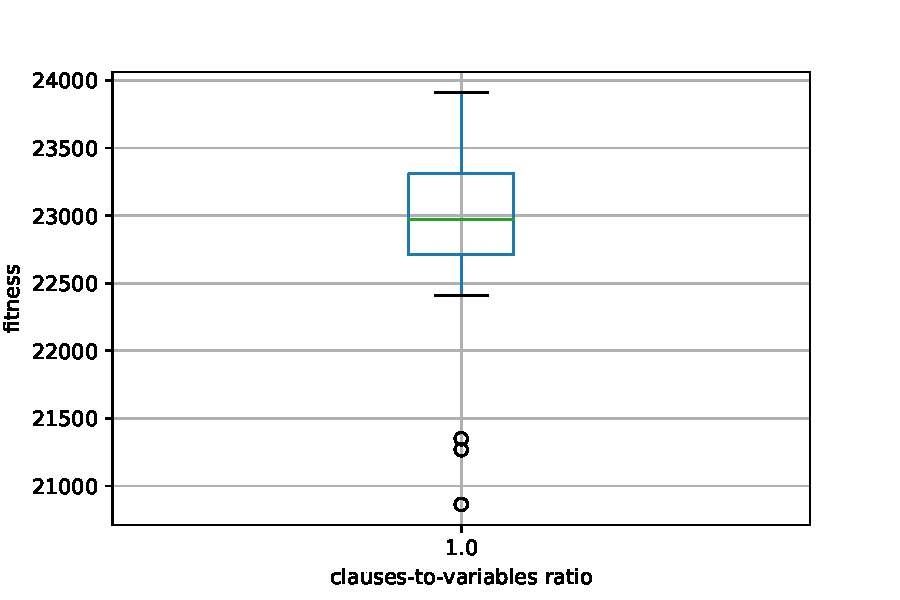
\includegraphics[width=\columnwidth]{figs/basic-boxplot}}
\caption{Boxplot of 30 best fitness values obtained on easy instance found
by genetic algorithm with basic parameters.}
\label{basic-boxplot}
\end{center}
\vskip -0.2in
\end{figure}

\begin{figure}[ht]
\vskip 0.2in
\begin{center}
\centerline{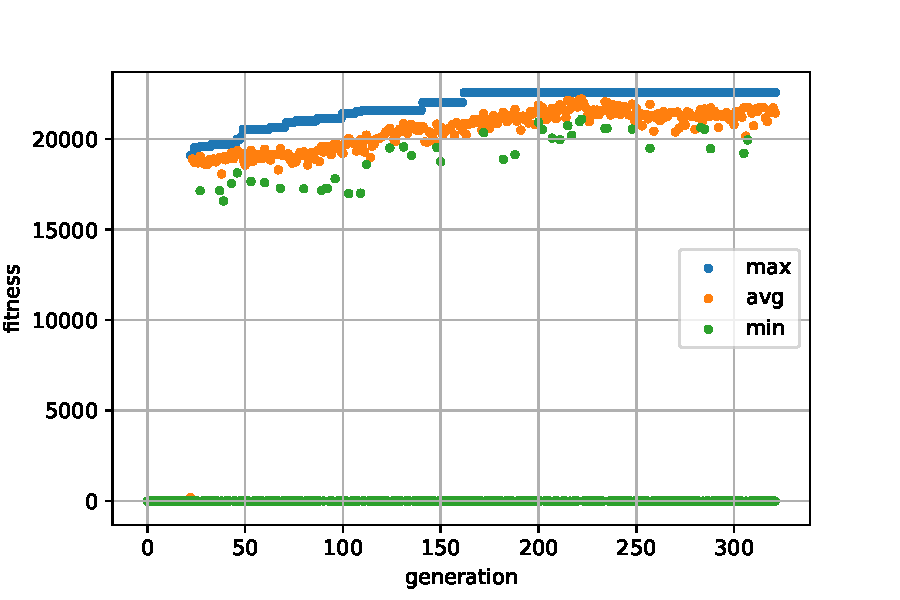
\includegraphics[width=\columnwidth]{figs/basic-progress}}
\caption{Fitness progress over generations of basic genetic algorithm on
easy instance. The algorithm is able to find satisfiable assignment soon.
On the other hand there is almost no exploration.
It almost seems that the algorithm is only exploiting one satisfiable solution.}
\label{basic-progress}
\end{center}
\vskip -0.2in
\end{figure}

\subsection{Selection}

One problem which prevents exploration might be roulette selection
because as soon as satisfiable individual is found
it is very unlikely to select unsatisfiable individual during selection
due to very high fitness in comparison with the individual with negative fitness.
Therefore tournament selection might explore more.

Table~\ref{result-table} show that indeed this can significantly improve
success rate but for the instances with clauses-to-variable ratio of 3.24
and 4.36 it is hard to find a satisfiable assignments.

\subsection{Crossover and Mutation}

Proposed in~\cite{park1995} crossover is considered marginal.
Therefore an experiment with crossover rate 0.0 and higher mutation rate 0.01
is carried out.

As shown in table~\ref{result-table} this really improves success rate even
for the most of second hardest instances.
On contrary the performance for the hardest instances is very bad but the
number of unsatisfied clauses goes slowly to 0.

In spite of the fact the performance on the hardest instances
this work is not concern with MAX-SAT but with weighted 3-SAT problem
so robustness in respect to this problem should be evaluated.

\section{Conclusion}

% In the unusual situation where you want a paper to appear in the
% references without citing it in the main text, use \nocite
%\nocite{langley00}

\bibliography{sat-report}
\bibliographystyle{icml2018}

\end{document}

% This document was modified from the file originally made available by
% Pat Langley and Andrea Danyluk for ICML-2K. This version was created
% by Iain Murray in 2018. It was modified from a version from Dan Roy in
% 2017, which was based on a version from Lise Getoor and Tobias
% Scheffer, which was slightly modified from the 2010 version by
% Thorsten Joachims & Johannes Fuernkranz, slightly modified from the
% 2009 version by Kiri Wagstaff and Sam Roweis's 2008 version, which is
% slightly modified from Prasad Tadepalli's 2007 version which is a
% lightly changed version of the previous year's version by Andrew
% Moore, which was in turn edited from those of Kristian Kersting and
% Codrina Lauth. Alex Smola contributed to the algorithmic style files.
